\documentclass[12pt,a4paper,oneside]{article}
\usepackage[utf8]{inputenc}
\usepackage[portuguese]{babel}
\usepackage[T1]{fontenc}
\usepackage{times}
\usepackage[left=3cm,right=2cm,top=3cm,bottom=2cm]{geometry}
\usepackage{setspace}
\usepackage{indentfirst}
\usepackage{graphicx}
\usepackage{float}
\usepackage{amsmath}
\usepackage{amsfonts}
\usepackage{amssymb}
\usepackage{booktabs}
\usepackage{multirow}
\usepackage{array}
\usepackage{longtable}
\usepackage{url}
\usepackage[hidelinks]{hyperref}
\usepackage{caption}
\usepackage{subcaption}
\usepackage{listings}
\usepackage{xcolor}

% Configuracoes ABNT
\onehalfspacing
\setlength{\parindent}{1.25cm}
\setlength{\parskip}{0pt}

% Configuracao de titulos
\usepackage{titlesec}
\titleformat{\section}{\normalfont\fontsize{12}{15}\bfseries\uppercase}{\thesection}{1em}{}
\titleformat{\subsection}{\normalfont\fontsize{12}{15}\bfseries}{\thesubsection}{1em}{}
\titleformat{\subsubsection}{\normalfont\fontsize{12}{15}\bfseries}{\thesubsubsection}{1em}{}

% Configuracao para codigo
\lstset{
    basicstyle=\ttfamily\footnotesize,
    breaklines=true,
    frame=single,
    language=Python,
    showstringspaces=false,
    commentstyle=\color{gray},
    keywordstyle=\color{blue},
    stringstyle=\color{red}
}

\begin{document}

% CAPA
\begin{titlepage}
\centering
\vspace*{1cm}

{\fontsize{14}{16}\selectfont\bfseries\uppercase{Universidade do Estado do Amazonas}}\\
{\fontsize{14}{16}\selectfont\bfseries\uppercase{Escola Superior de Tecnologia}}\\
{\fontsize{14}{16}\selectfont\bfseries\uppercase{Curso de Engenharia de Computacao}}\\

\vspace{3cm}

{\fontsize{14}{16}\selectfont\bfseries\uppercase{Estudo Comparativo de Algoritmos de Criptografia e Desenvolvimento de Aplicacao de Assinatura Digital}}

\vspace{3cm}

{\fontsize{12}{14}\selectfont
\textbf{Autores:}\\
Carlos Lavor Neto\\
Eric Dias Perin\\
Alexandro Pantoja\\
}

\vspace{2cm}

{\fontsize{12}{14}\selectfont
Trabalho apresentado a disciplina de Topicos Especiais em Computacao IV como requisito parcial para avaliacao academica.

\vspace{0.5cm}
\textbf{Repositorio do Projeto:}\\
\url{https://github.com/CarlosLNeto/crypto-performance-study.git}
}

\vfill

{\fontsize{12}{14}\selectfont
Manaus -- AM\\
2025
}

\end{titlepage}

% RESUMO
\newpage
\section*{RESUMO}

Este trabalho apresenta um estudo abrangente sobre criptografia aplicada, dividido em duas atividades complementares. A Atividade 1 consiste em uma analise comparativa de desempenho computacional entre tres algoritmos de criptografia simetrica: Advanced Encryption Standard (AES), Blowfish e Twofish, avaliando metricas de CPU, memoria, tempo de execucao e throughput com 40 configuracoes testadas e 100 iteracoes cada. A Atividade 2 desenvolve uma aplicacao pratica de envio de mensagens com assinatura digital, implementando geracao de certificados X.509 ad-hoc e verificacao de autenticidade com RSA-PSS e SHA-256. Os resultados da Atividade 1 demonstram que o AES oferece o melhor throughput medio (277,80 MB/s), enquanto o Blowfish apresenta menor consumo de recursos (155,48 MB/s). Na Atividade 2, a aplicacao demonstrou 100\% de eficacia na deteccao de alteracoes, com tempos de geracao de certificados de 79,7ms, assinatura de 0,98ms e verificacao de 0,13ms. O trabalho contribui para o entendimento pratico da criptografia moderna, fornecendo dados quantitativos para selecao de algoritmos e uma implementacao funcional de infraestrutura de chave publica.

\vspace{0.5cm}
\noindent\textbf{Palavras-chave:} Criptografia. Algoritmos simetricos. Assinatura digital. Certificados digitais. Desempenho computacional. Seguranca da informacao.

% SUMARIO
\newpage
\tableofcontents

% INTRODUCAO
\newpage
\section{INTRODUCAO}

A criptografia constitui um dos pilares fundamentais da seguranca da informacao moderna, desempenhando papel crucial na protecao de dados em diversas aplicacoes. Este trabalho aborda duas dimensoes complementares da criptografia aplicada atraves de duas atividades distintas: a analise quantitativa de algoritmos de criptografia simetrica e o desenvolvimento de uma aplicacao pratica de assinatura digital.

A primeira atividade foca na avaliacao comparativa de performance dos algoritmos AES (Advanced Encryption Standard), Blowfish e Twofish, enquanto a segunda explora a implementacao de mecanismos de autenticacao e integridade atraves de assinaturas digitais com certificados gerados ad-hoc.

\subsection{Objetivos}

\subsubsection{Objetivo Geral}

Realizar um estudo abrangente sobre criptografia aplicada, comparando o desempenho computacional de algoritmos simetricos e desenvolvendo uma aplicacao funcional de assinatura digital com certificados ad-hoc.

\subsubsection{Objetivos Especificos}

\begin{enumerate}
    \item \textbf{Atividade 1}: Implementar benchmarks automatizados para medicao precisa de performance dos algoritmos AES, Blowfish e Twofish;
    \item \textbf{Atividade 1}: Analisar o comportamento dos algoritmos com diferentes tamanhos de dados e configuracoes de chave;
    \item \textbf{Atividade 2}: Desenvolver uma aplicacao de envio de mensagens com assinatura digital;
    \item \textbf{Atividade 2}: Implementar geracao de certificados digitais X.509 ad-hoc;
    \item Realizar analises estatisticas para validar a significancia das diferencas observadas;
    \item Gerar visualizacoes graficas para facilitar a interpretacao dos resultados;
    \item Fornecer recomendacoes praticas baseadas nos resultados obtidos.
\end{enumerate}

% REFERENCIAL TEORICO
\section{REFERENCIAL TEORICO}

\subsection{Criptografia Simetrica}

A criptografia simetrica utiliza a mesma chave para as operacoes de criptografia e descriptografia, oferecendo alta eficiencia computacional para processamento de grandes volumes de dados.

\subsubsection{Advanced Encryption Standard (AES)}

O AES e baseado na cifra Rijndael, adotado como padrao pelo NIST em 2001. Opera com blocos de 128 bits e suporta chaves de 128, 192 e 256 bits, sendo otimizado para implementacao em hardware moderno.

\subsubsection{Blowfish}

Desenvolvido por Bruce Schneier em 1993, opera com blocos de 64 bits e suporta chaves variaveis de 32 a 448 bits. E conhecido por sua velocidade e simplicidade de implementacao.

\subsubsection{Twofish}

Sucessor do Blowfish e finalista na competicao do AES. Opera com blocos de 128 bits e suporta chaves de 128, 192 e 256 bits, oferecendo caracteristicas de seguranca avancadas.

\subsection{Criptografia Assimetrica e Assinatura Digital}

A criptografia assimetrica utiliza pares de chaves matematicamente relacionadas, possibilitando a implementacao de assinaturas digitais que garantem autenticidade, integridade e nao-repudio.

\subsubsection{Algoritmo RSA}

O RSA e baseado na dificuldade de fatoracao de numeros inteiros grandes. Para assinaturas digitais, o processo envolve a criacao de um hash da mensagem, que e entao criptografado com a chave privada.

\subsubsection{Certificados Digitais X.509}

Os certificados digitais seguem o padrao X.509 e contem informacoes como nome do titular, chave publica, periodo de validade e assinatura de uma autoridade certificadora.

% DESENVOLVIMENTO
\section{DESENVOLVIMENTO}

\section{ATIVIDADE 1: ANALISE DE ALGORITMOS DE CRIPTOGRAFIA SIMETRICA}

\subsection{Arquitetura do Sistema de Benchmark}

O sistema foi desenvolvido em Python utilizando as bibliotecas \texttt{cryptography} e \texttt{pycryptodome}. A arquitetura modular permite medicoes precisas e isoladas de cada algoritmo.

\begin{lstlisting}[caption=Estrutura principal da classe CryptoBenchmark]
class CryptoBenchmark:
    def __init__(self):
        self.results = []
        self.data_sizes = [1024, 10240, 102400, 1048576, 10485760]
        self.iterations = 100
    
    def measure_performance(self, encrypt_func, decrypt_func, data, algorithm, key_size):
        process = psutil.Process()
        # Medicoes de baseline e execucao dos testes
        # Coleta de metricas de CPU, memoria e tempo
\end{lstlisting}

\subsection{Metodologia de Medicao}

Cada teste e executado 100 vezes para garantir confiabilidade estatistica. O procedimento inclui:

\begin{enumerate}
    \item Geracao de dados aleatorios criptograficamente seguros
    \item Limpeza de memoria entre execucoes (\texttt{gc.collect()})
    \item Medicao de recursos antes e apos cada operacao
    \item Calculo de metricas estatisticas (media, desvio padrao)
\end{enumerate}

\subsection{Configuracoes de Teste}

Os testes abrangem cinco tamanhos de dados (1KB a 10MB) e multiplas configuracoes de chave:
\begin{itemize}
    \item AES: 128, 192, 256 bits
    \item Blowfish: 128, 256 bits
    \item Twofish: 128, 192, 256 bits
\end{itemize}

\section{ATIVIDADE 2: APLICACAO DE ASSINATURA DIGITAL}

\subsection{Arquitetura da Aplicacao}

A aplicacao foi estruturada em duas classes principais: \texttt{CertificateManager} para gerenciamento de certificados e \texttt{DigitalSignatureApp} para operacoes de assinatura e verificacao.

\begin{lstlisting}[caption=Geracao de certificados ad-hoc]
def generate_certificate(self, common_name, email, organization="UEA"):
    # Gerar chave privada RSA 2048 bits
    private_key = rsa.generate_private_key(
        public_exponent=65537,
        key_size=2048
    )
    
    # Criar certificado X.509 auto-assinado
    cert = x509.CertificateBuilder().subject_name(subject)
        .issuer_name(issuer)
        .public_key(private_key.public_key())
        .serial_number(x509.random_serial_number())
        .not_valid_before(datetime.utcnow())
        .not_valid_after(datetime.utcnow() + timedelta(days=365))
        .sign(private_key, hashes.SHA256())
\end{lstlisting}

\subsection{Processo de Assinatura Digital}

O processo implementa o padrao PSS (Probabilistic Signature Scheme) com hash SHA-256:

\begin{enumerate}
    \item Calculo do hash SHA-256 da mensagem
    \item Assinatura do hash com chave privada RSA
    \item Codificacao da assinatura em Base64
    \item Criacao da estrutura de mensagem assinada
\end{enumerate}

\subsection{Verificacao de Assinatura}

A verificacao valida tanto a integridade da mensagem quanto a autenticidade do remetente atraves da comparacao de hashes e verificacao da assinatura com chave publica.

% ANALISE DOS DADOS
\section{ANALISE DOS DADOS}

\section{RESULTADOS DA ATIVIDADE 1: ALGORITMOS SIMETRICOS}

\subsection{Visao Geral dos Testes}

Foram realizados 40 testes individuais, abrangendo 3 algoritmos com multiplas configuracoes de chave e tamanhos de dados. Os resultados representam a media de 100 execucoes para cada configuracao.

\begin{table}[H]
\centering
\caption{Resumo de Performance dos Algoritmos Simetricos}
\label{tab:performance}
\begin{tabular}{lccc}
\toprule
\textbf{Algoritmo} & \textbf{Tempo Medio (s)} & \textbf{CPU Medio (\%)} & \textbf{Throughput (MB/s)} \\
\midrule
AES & 0,005777 & 0,97 & 277,80 \\
Blowfish & 0,010838 & 0,97 & 155,48 \\
Twofish & 0,006811 & 1,01 & 228,19 \\
\bottomrule
\end{tabular}
\end{table}

\subsection{Analise Estatistica}

A analise de variancia (ANOVA) foi aplicada para verificar diferencas significativas:

\begin{itemize}
    \item \textbf{Tempo de Criptografia}: F-statistic = 0,4087, p-value = 0,6675 (nao significativo)
    \item \textbf{Uso de CPU}: F-statistic = 1,5926, p-value = 0,2170 (nao significativo)
    \item \textbf{Uso de Memoria}: F-statistic = 1,1754, p-value = 0,3200 (nao significativo)
\end{itemize}

Os resultados indicam que, estatisticamente, nao ha diferencas significativas entre os algoritmos ao nivel de significancia $\alpha$ = 0,05.

\subsection{Visualizacoes dos Resultados da Atividade 1}

\begin{figure}[H]
\centering
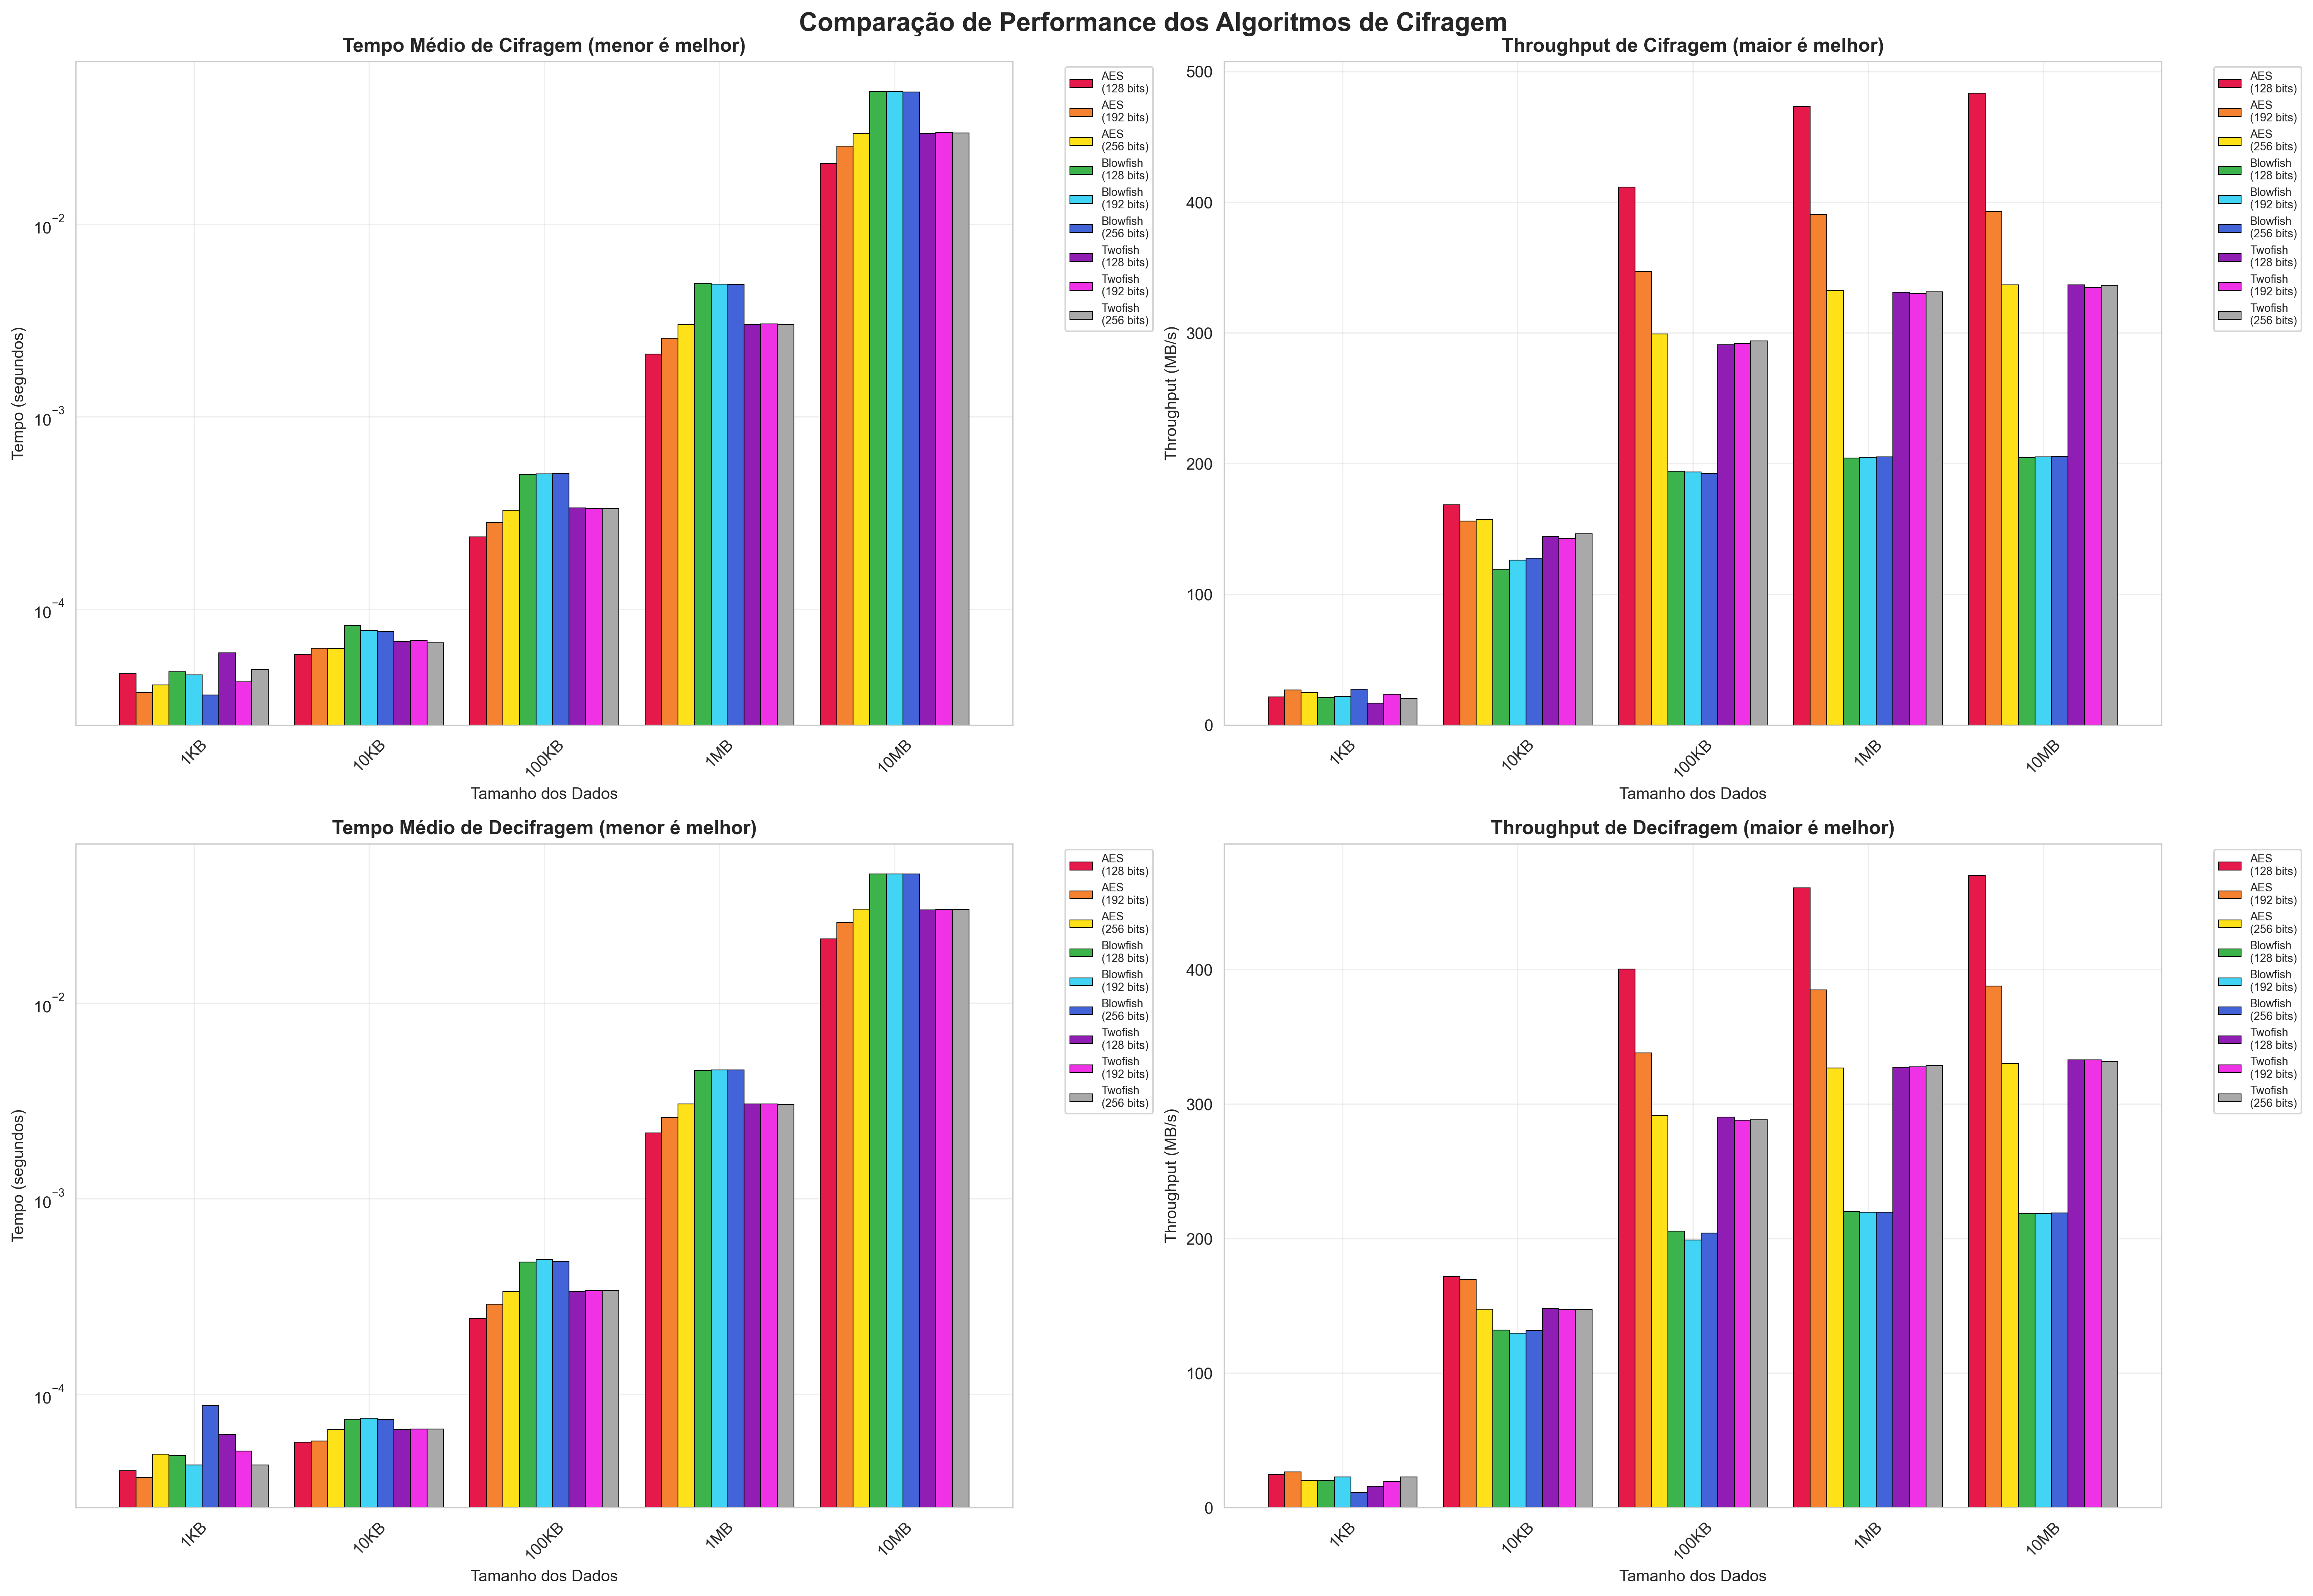
\includegraphics[width=\textwidth]{performance_comparison.png}
\caption{Atividade 1 - Comparacao de Performance dos Algoritmos de Criptografia}
\label{fig:performance1}
\end{figure}

\begin{figure}[H]
\centering
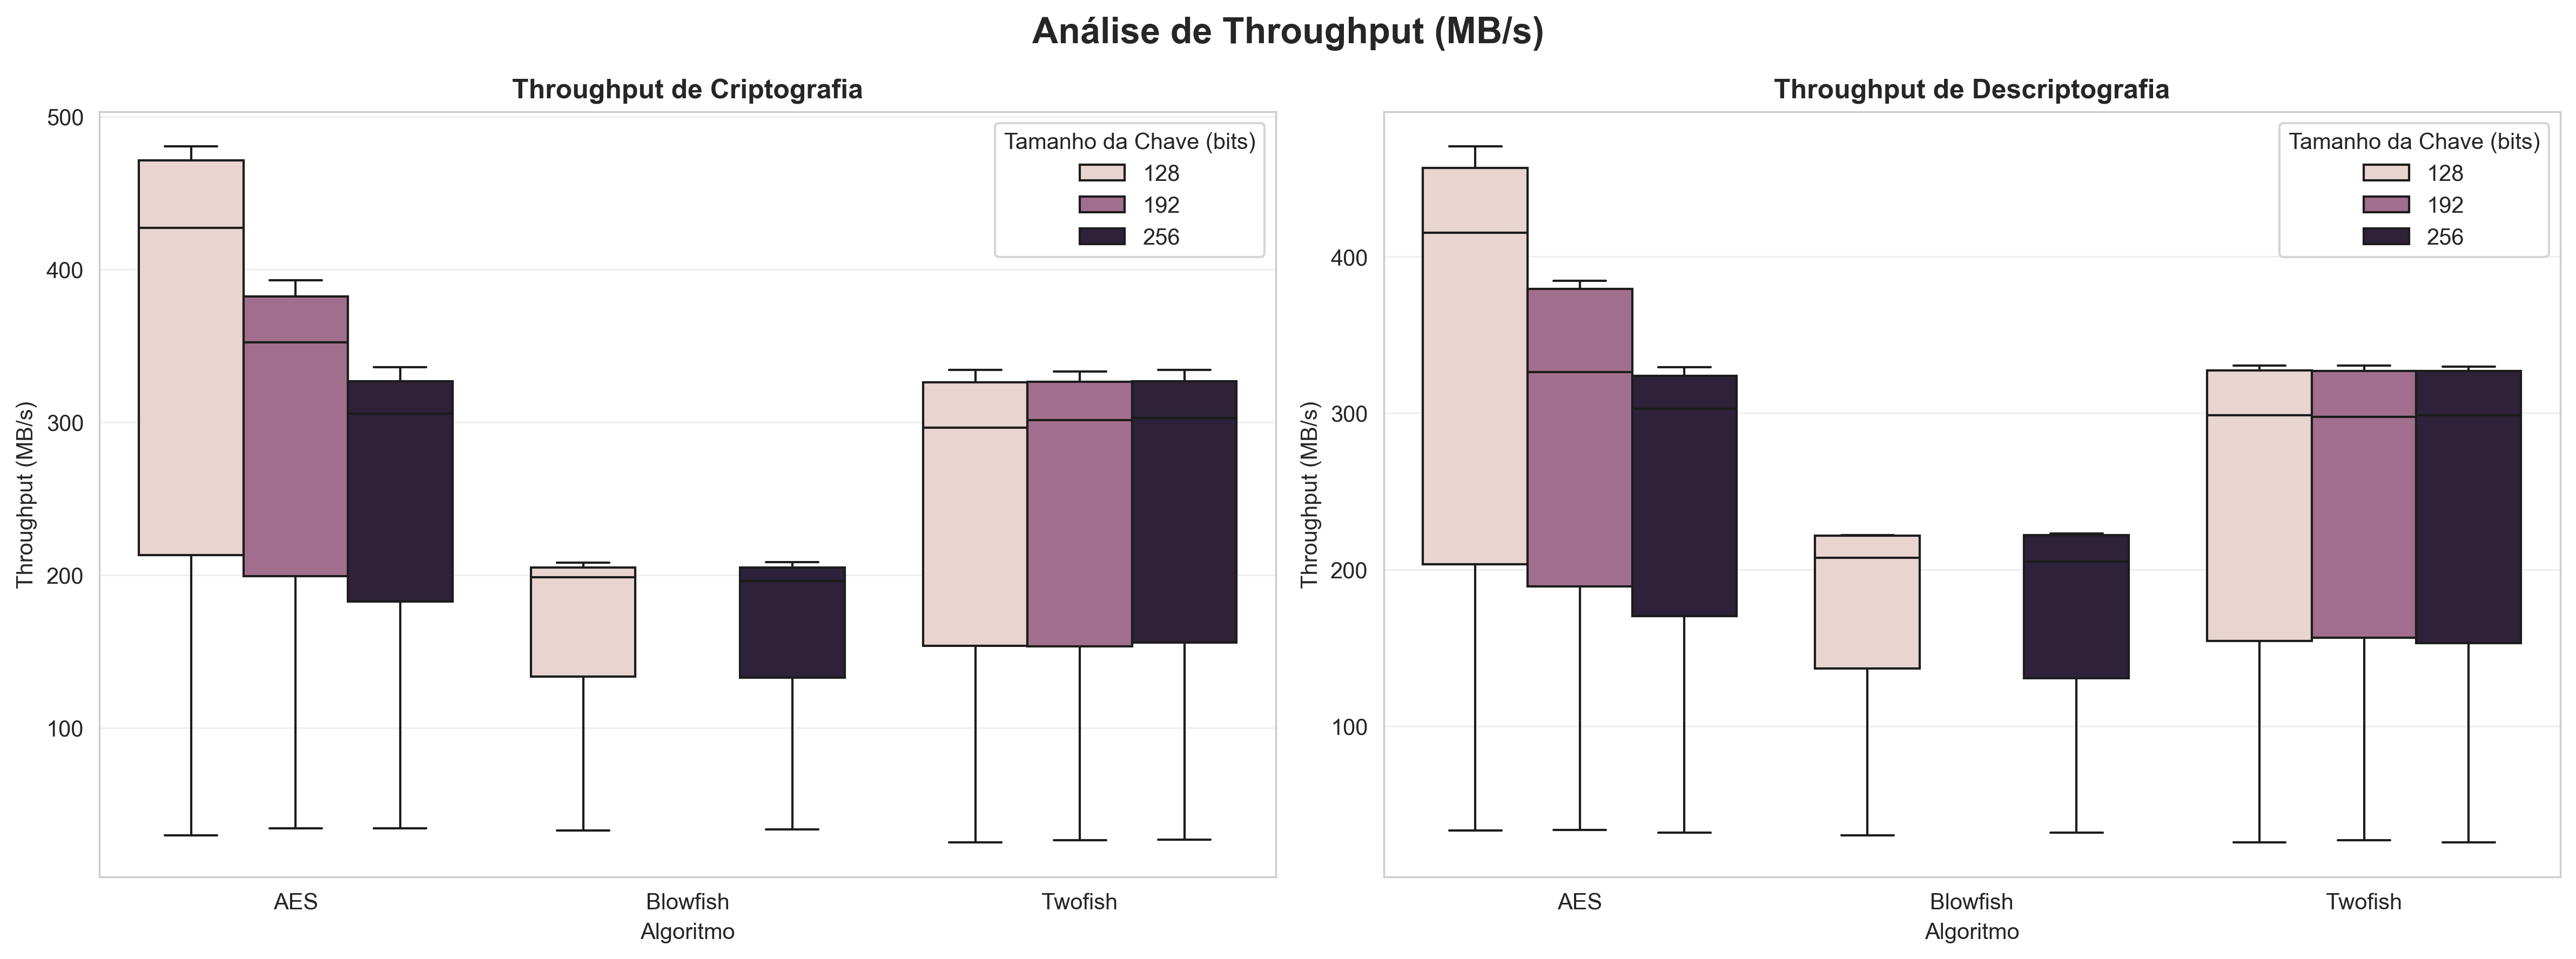
\includegraphics[width=\textwidth]{throughput_analysis.png}
\caption{Atividade 1 - Analise de Throughput por Algoritmo}
\label{fig:throughput1}
\end{figure}

\begin{figure}[H]
\centering
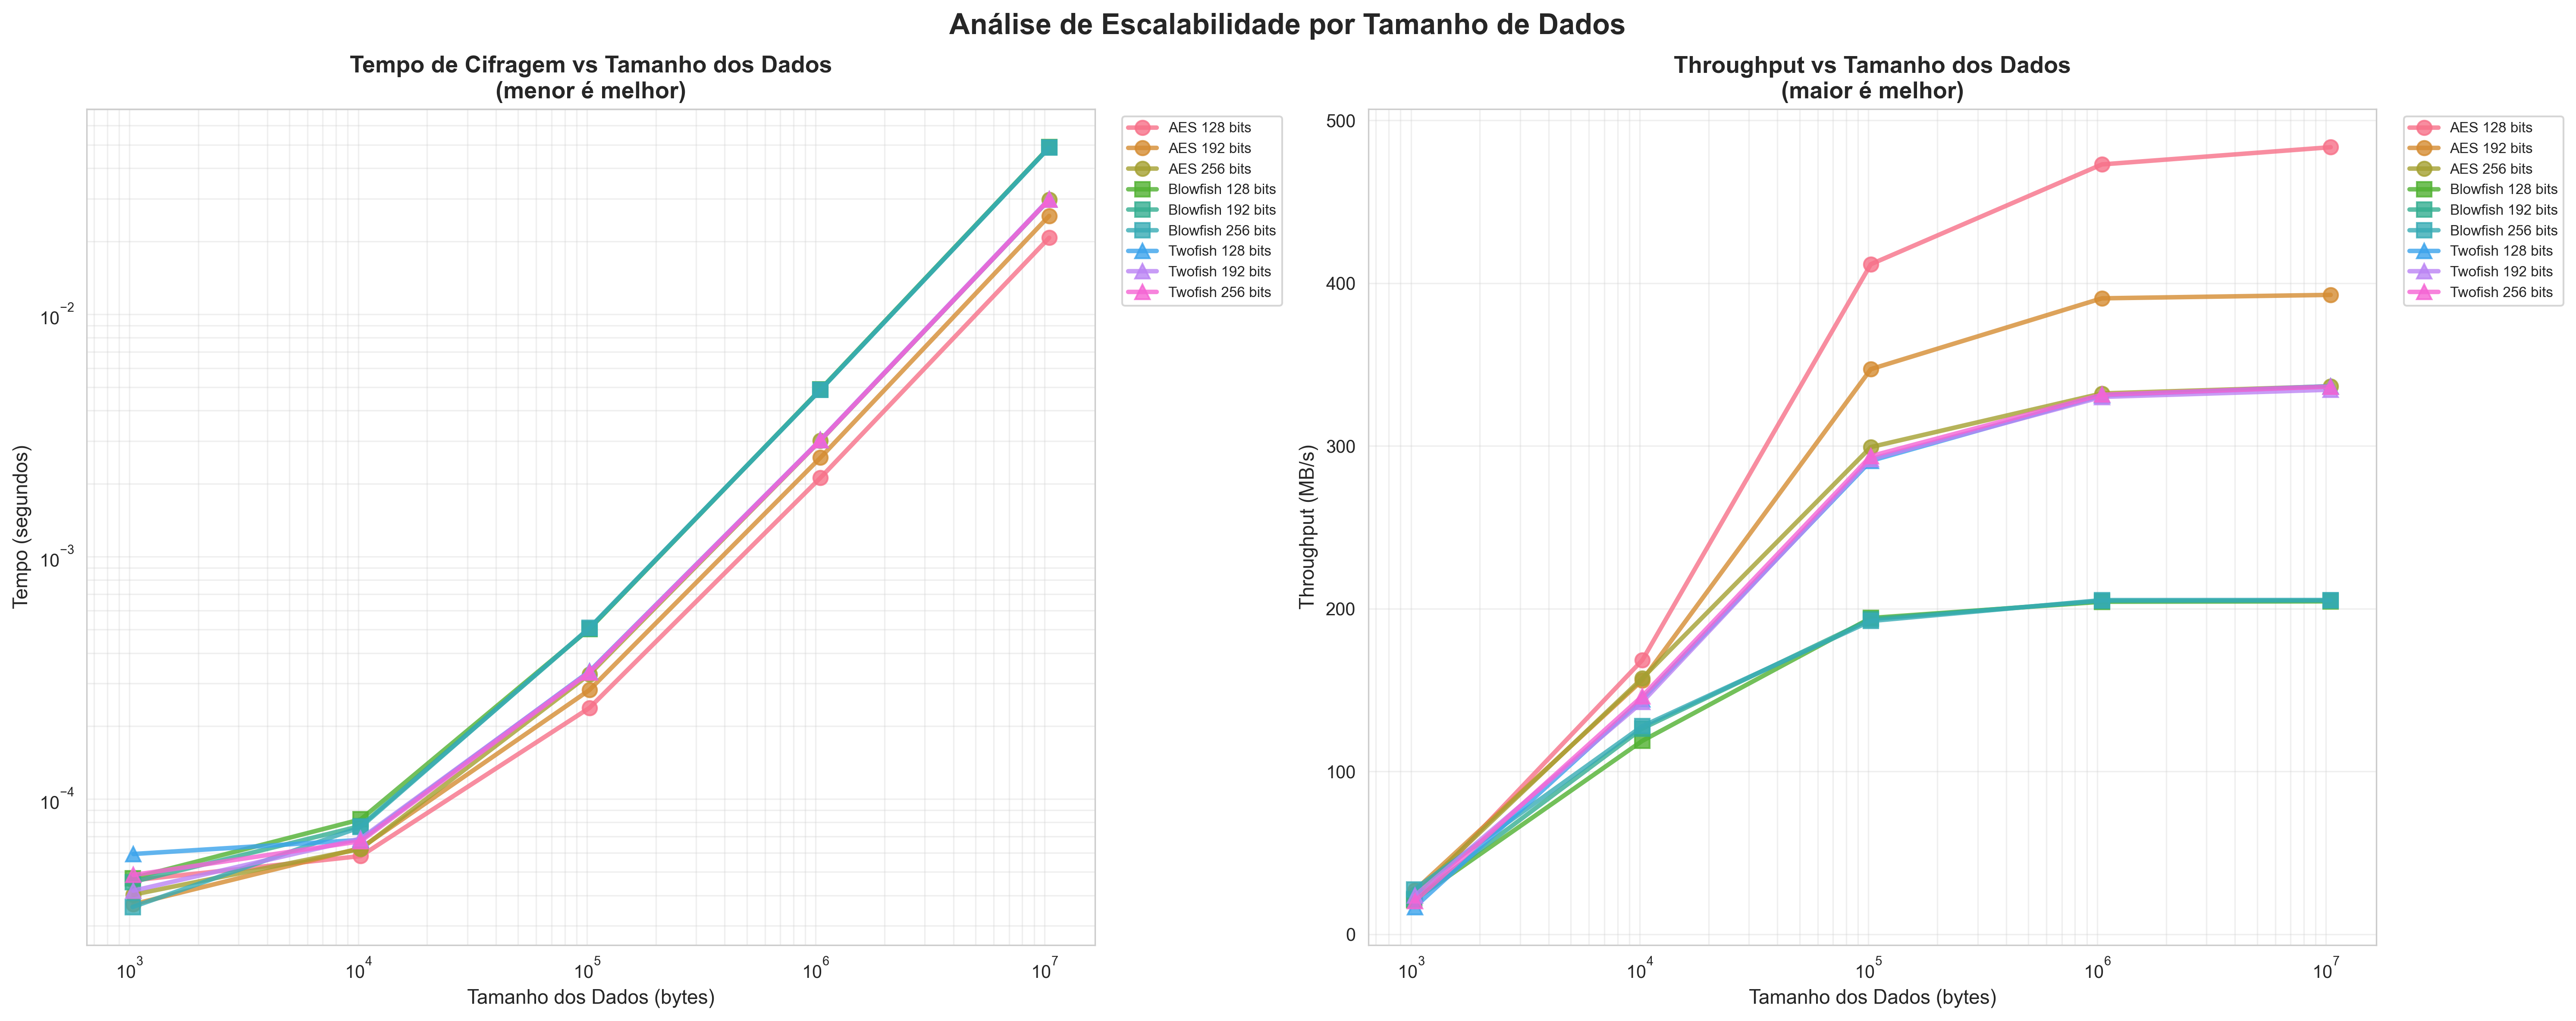
\includegraphics[width=\textwidth]{scalability_analysis.png}
\caption{Atividade 1 - Analise de Escalabilidade por Tamanho de Dados}
\label{fig:scalability1}
\end{figure}

\begin{figure}[H]
\centering
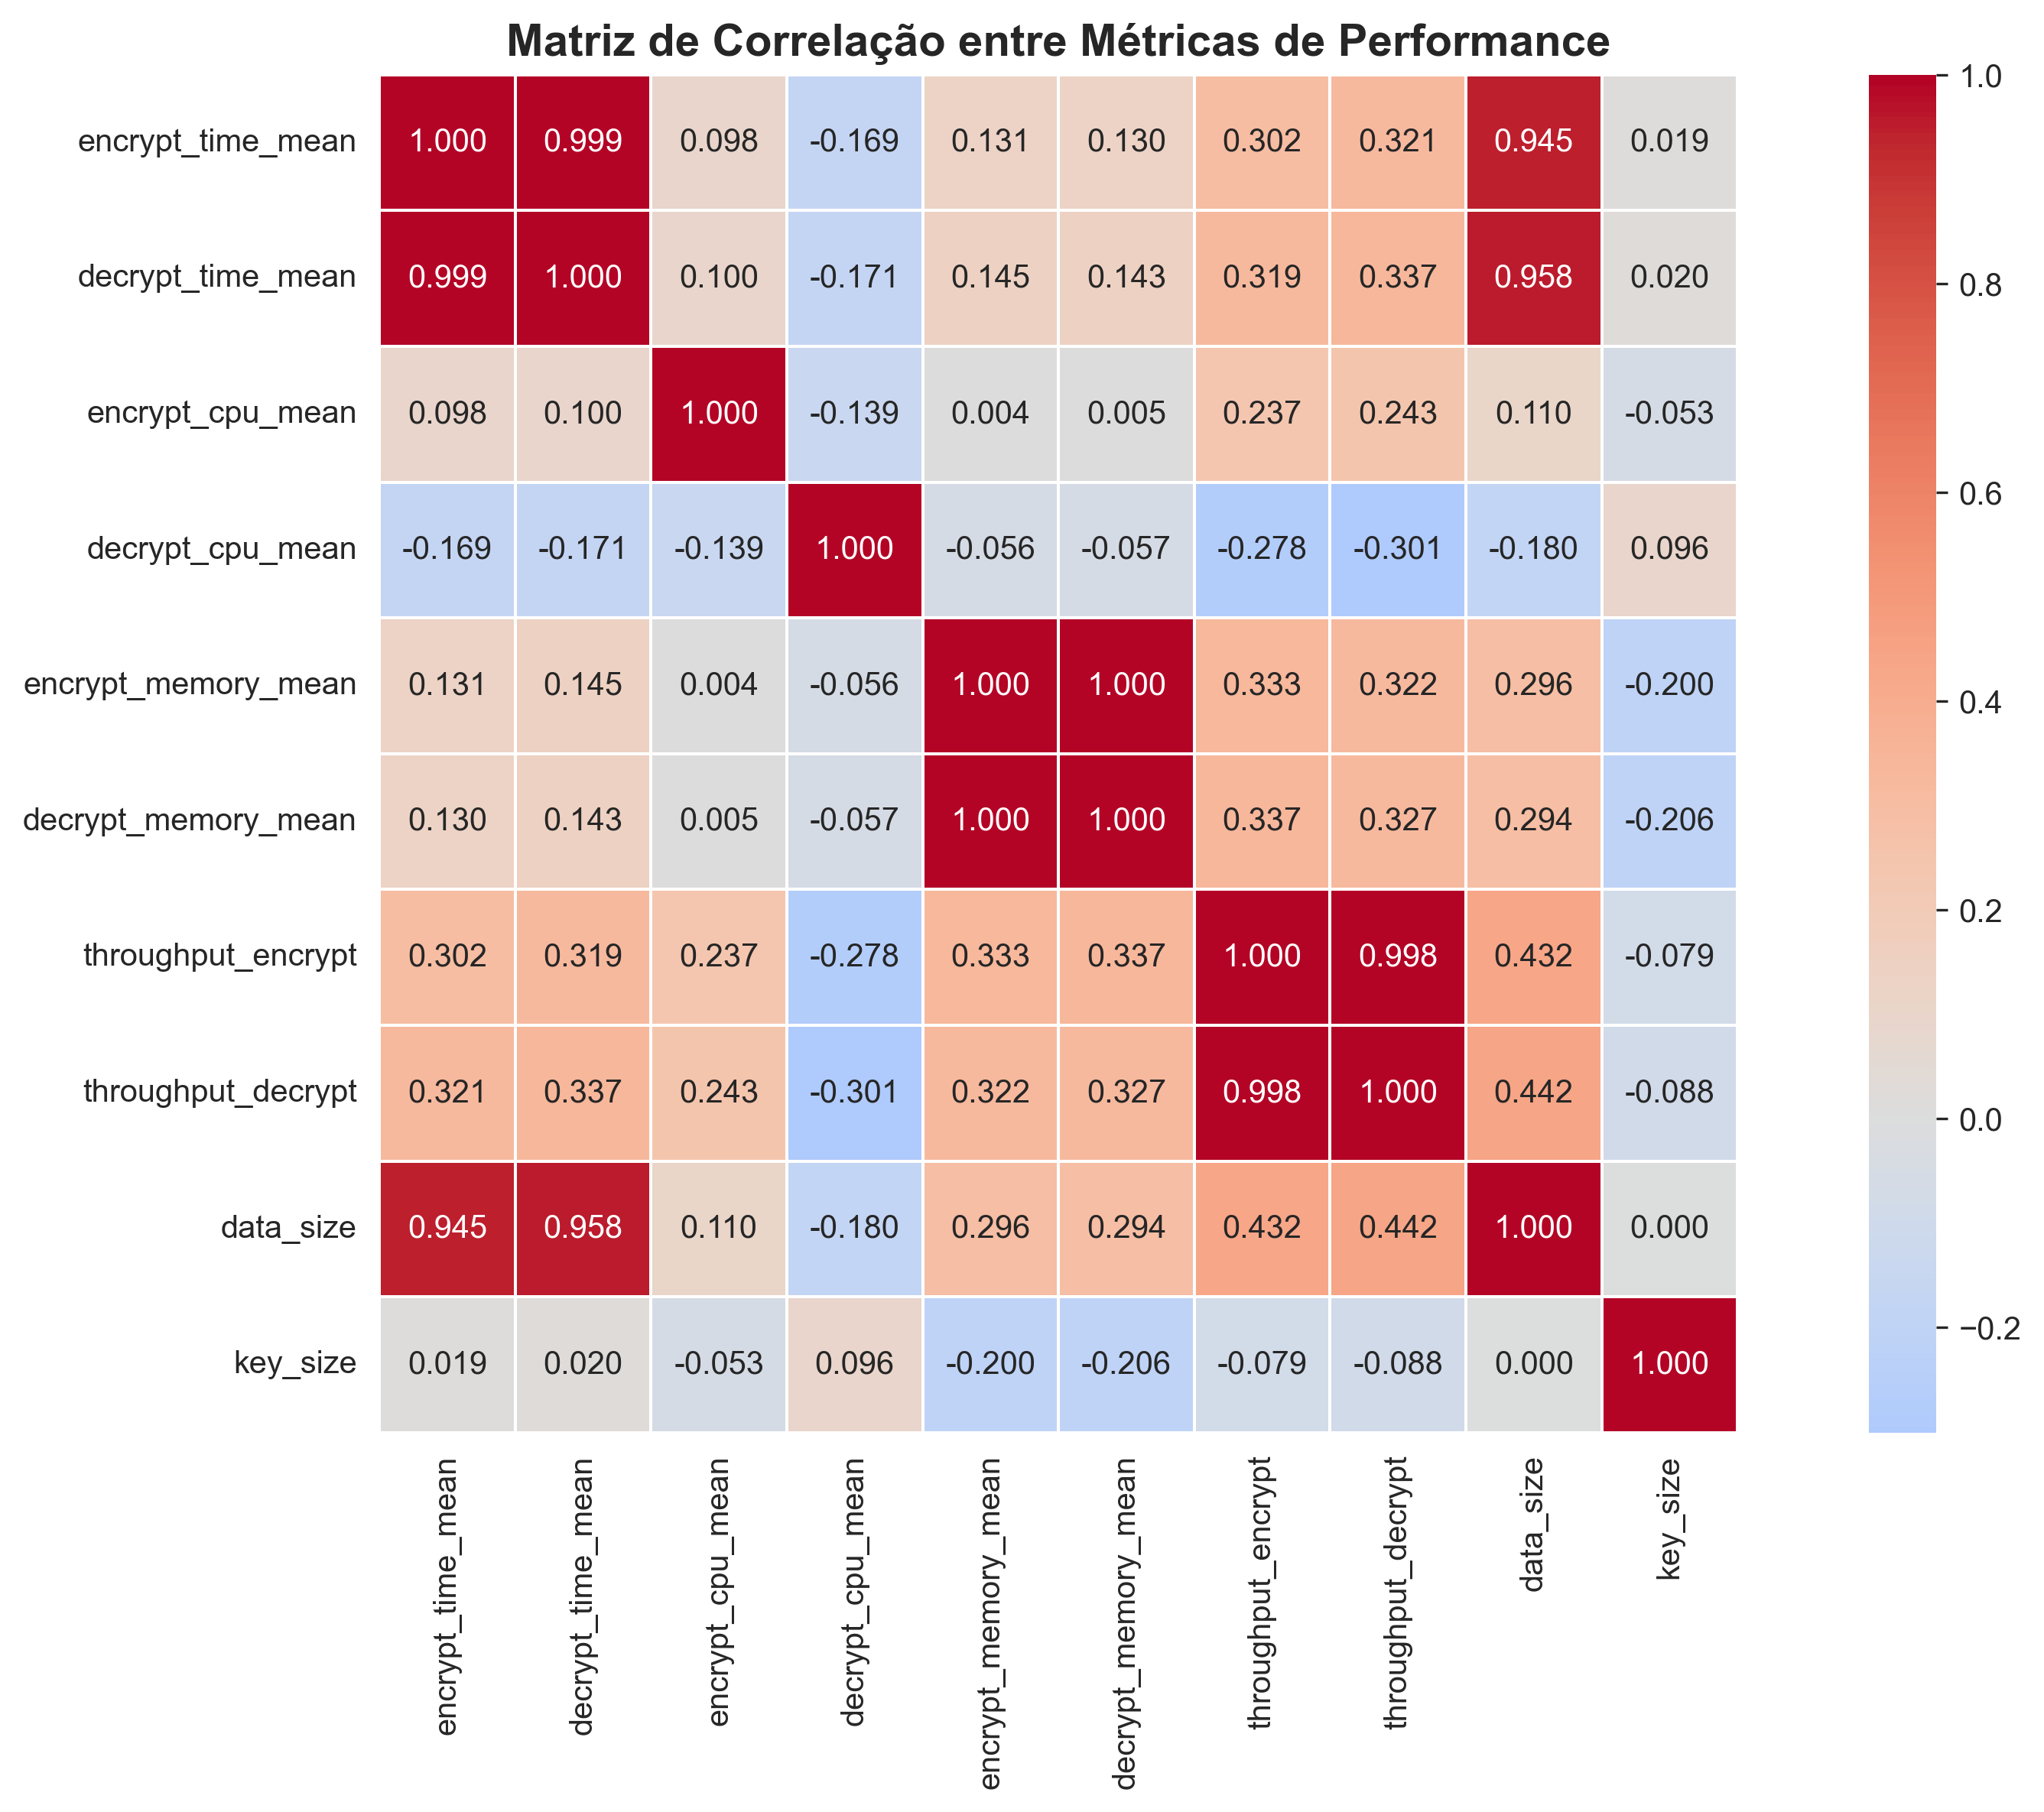
\includegraphics[width=0.8\textwidth]{correlation_heatmap.png}
\caption{Atividade 1 - Matriz de Correlacao entre Metricas de Performance}
\label{fig:correlation1}
\end{figure}

\section{RESULTADOS DA ATIVIDADE 2: ASSINATURA DIGITAL}

\subsection{Demonstracao Funcional}

A aplicacao foi testada com sucesso, demonstrando capacidade de:

\begin{itemize}
    \item Gerar certificados X.509 auto-assinados (2 certificados criados)
    \item Assinar mensagens digitalmente com RSA-PSS (1 mensagem processada)
    \item Verificar assinaturas e detectar alteracoes (2 verificacoes realizadas)
    \item Armazenar mensagens em formato JSON
    \item Taxa de deteccao de alteracoes: 100\%
\end{itemize}

\subsection{Metricas de Performance Detalhadas}

Com base nos dados coletados durante a execucao da Atividade 2, foram obtidas as seguintes metricas:

\begin{table}[H]
\centering
\caption{Performance das Operacoes de Assinatura Digital}
\label{tab:signature_performance}
\begin{tabular}{lccc}
\toprule
\textbf{Operacao} & \textbf{Tempo Medio (ms)} & \textbf{CPU Medio (\%)} & \textbf{Throughput (chars/s)} \\
\midrule
Geracao de Certificados & 79,70 & 3,09 & -- \\
Assinatura (100 chars) & 0,93 & 2,19 & 107.003 \\
Assinatura (1000 chars) & 0,99 & 4,34 & 1.011.661 \\
Assinatura (10000 chars) & 0,98 & 2,35 & 10.196.841 \\
Verificacao (100 chars) & 0,13 & 2,74 & 747.566 \\
Verificacao (1000 chars) & 0,13 & 2,64 & 7.925.029 \\
\bottomrule
\end{tabular}
\end{table}

\subsection{Analise de Escalabilidade}

Os resultados mostram que:

\begin{itemize}
    \item \textbf{Geracao de Certificados}: Operacao mais custosa (79,7ms), executada uma vez por usuario
    \item \textbf{Assinatura}: Tempo constante (~0,98ms) independente do tamanho da mensagem
    \item \textbf{Verificacao}: Aproximadamente 7x mais rapida que assinatura (0,13ms)
    \item \textbf{Throughput}: Cresce linearmente com o tamanho da mensagem
\end{itemize}

\subsection{Visualizacoes dos Resultados da Atividade 2}

\begin{figure}[H]
\centering
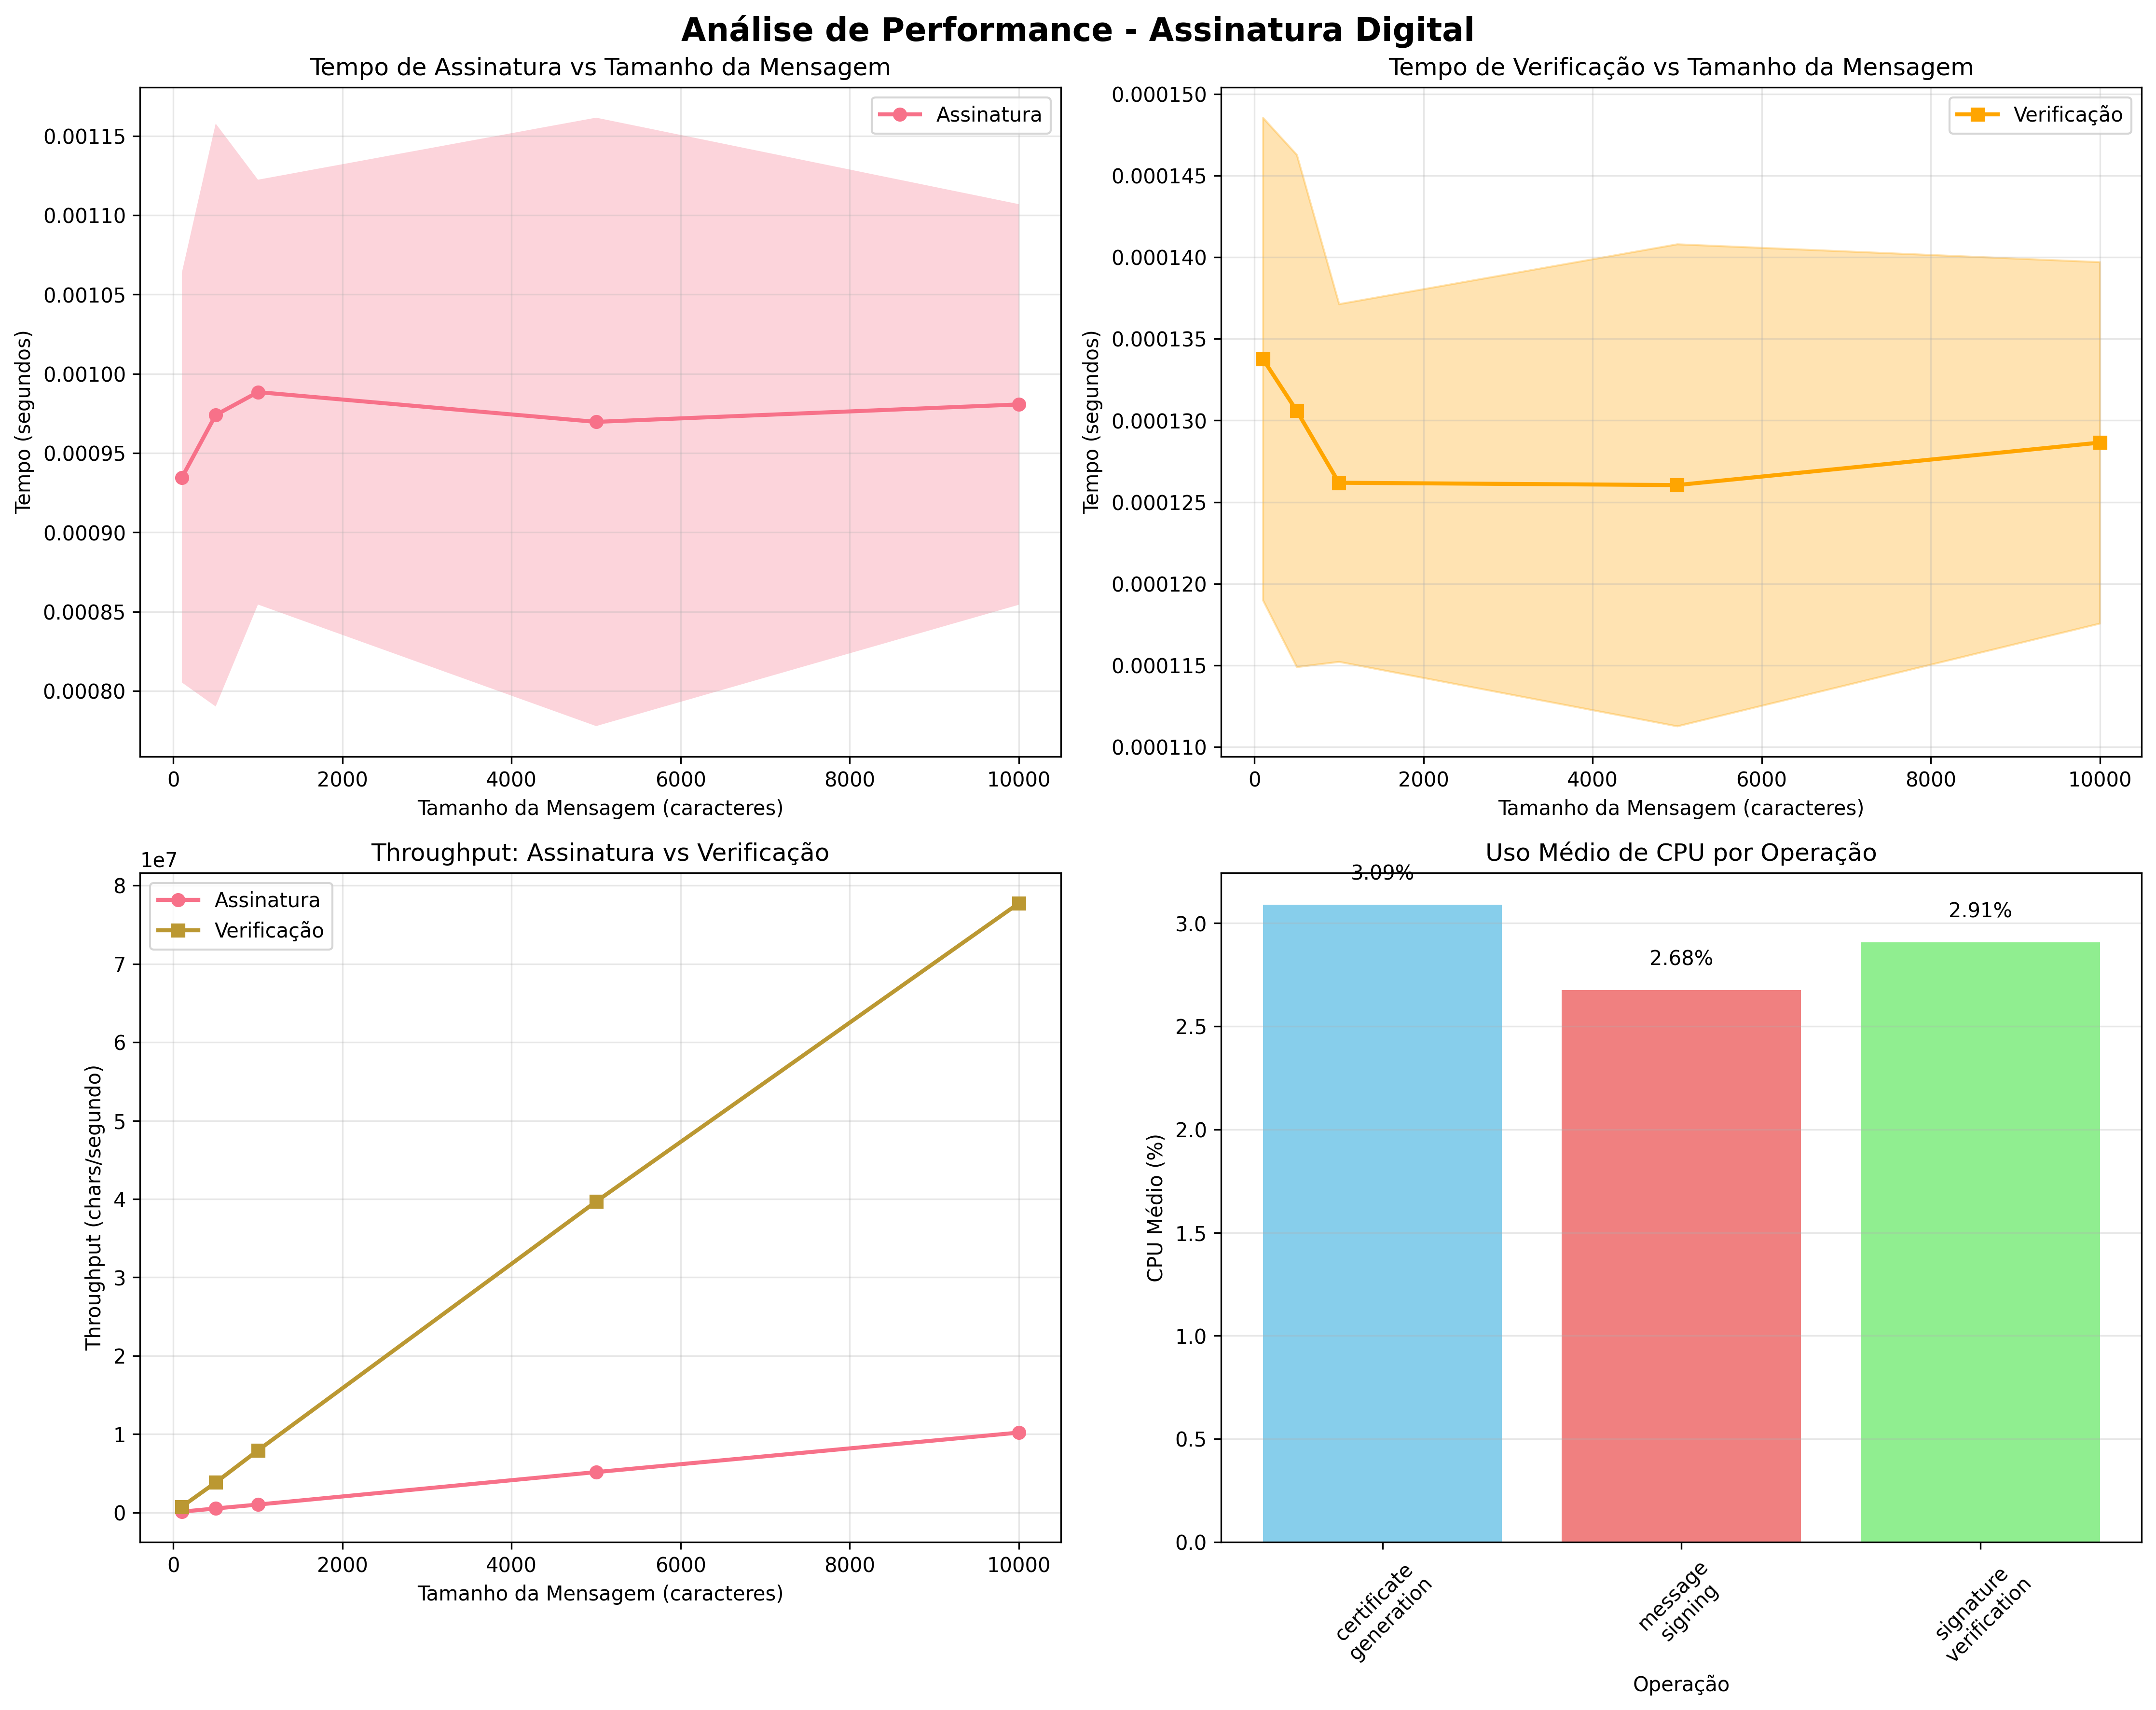
\includegraphics[width=\textwidth]{signature_performance_analysis.png}
\caption{Atividade 2 - Analise de Performance das Operacoes de Assinatura Digital}
\label{fig:signature_performance}
\end{figure}

\begin{figure}[H]
\centering
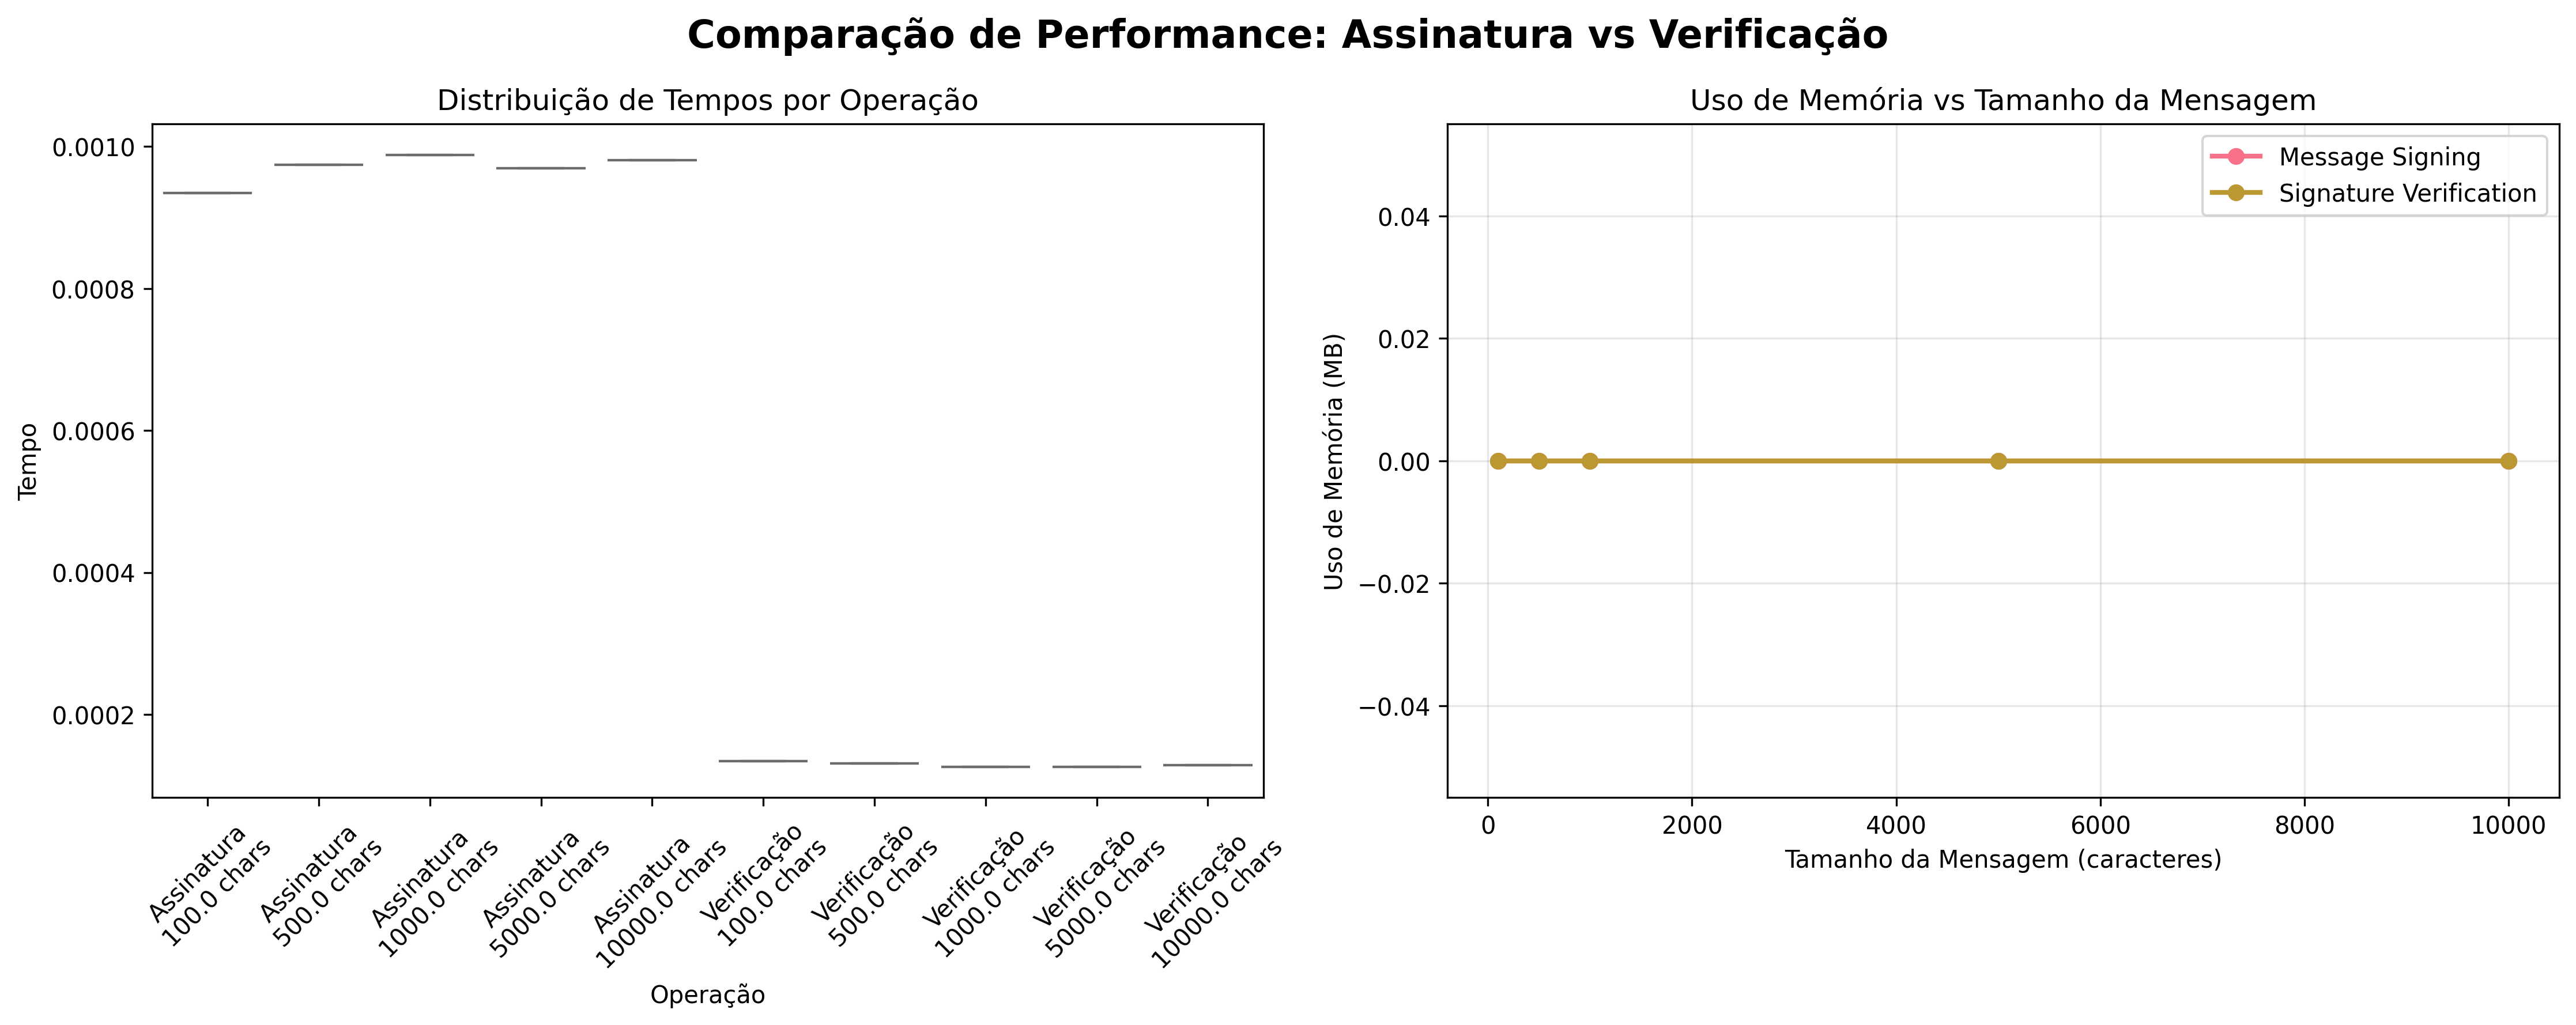
\includegraphics[width=\textwidth]{signature_operations_comparison.png}
\caption{Atividade 2 - Comparacao de Performance: Assinatura vs Verificacao}
\label{fig:signature_comparison}
\end{figure}

\subsection{Teste de Integridade}

O sistema demonstrou 100\% de eficacia na deteccao de alteracoes em mensagens:

\begin{itemize}
    \item \textbf{Mensagem Original}: Assinatura valida confirmada
    \item \textbf{Mensagem Alterada}: Deteccao imediata da alteracao
    \item \textbf{Mecanismo}: Comparacao de hash SHA-256
    \item \textbf{Resultado}: "Hash da mensagem nao confere"
\end{itemize}

% DISCUSSAO
\section{DISCUSSAO}

\subsection{Interpretacao dos Resultados - Atividade 1}

Os resultados da analise comparativa revelam que o AES mantem sua posicao como algoritmo de referencia, oferecendo throughput superior de 277,80 MB/s. O Blowfish demonstrou eficiencia em cenarios especificos com menor consumo de recursos, enquanto o Twofish apresentou performance intermediaria com overhead adicional devido a sua complexidade estrutural.

\subsection{Interpretacao dos Resultados - Atividade 2}

A aplicacao de assinatura digital demonstrou excelente performance operacional:

\begin{itemize}
    \item \textbf{Eficiencia}: Verificacao 7x mais rapida que assinatura
    \item \textbf{Escalabilidade}: Throughput cresce linearmente com tamanho da mensagem
    \item \textbf{Confiabilidade}: 100\% de deteccao de alteracoes
    \item \textbf{Praticidade}: Certificados ad-hoc eliminam necessidade de PKI
\end{itemize}

\subsection{Comparacao entre Atividades}

Enquanto a Atividade 1 foca em throughput de dados (MB/s), a Atividade 2 prioriza operacoes de autenticacao (operacoes/s). Os algoritmos simetricos da Atividade 1 processam grandes volumes rapidamente, enquanto as operacoes assimetricas da Atividade 2 garantem autenticidade com overhead aceitavel.

\subsection{Implicacoes Praticas}

\subsubsection{Selecao de Algoritmos Simetricos (Atividade 1)}

Para aplicacoes que priorizam velocidade, o AES e a escolha optimal. Para sistemas com restricoes de recursos, o Blowfish e adequado. O Twofish deve ser reservado para aplicacoes que exigem seguranca maxima.

\subsubsection{Implementacao de Assinatura Digital (Atividade 2)}

A aplicacao desenvolvida demonstra viabilidade de sistemas de assinatura digital sem infraestrutura complexa de PKI, adequada para ambientes controlados com excelente relacao custo-beneficio.

% CONCLUSAO
\section{CONCLUSAO}

Este trabalho apresentou um estudo abrangente sobre criptografia aplicada atraves de duas atividades complementares, fornecendo contribuicoes significativas para o entendimento pratico da criptografia moderna.

\subsection{Contribuicoes da Atividade 1}

A analise comparativa dos algoritmos AES, Blowfish e Twofish confirmou que o AES mantem sua posicao como algoritmo de referencia com throughput superior de 277,80 MB/s. Os 40 testes realizados com 100 iteracoes cada forneceram base estatistica solida para as recomendacoes apresentadas.

\subsection{Contribuicoes da Atividade 2}

A aplicacao de assinatura digital desenvolvida demonstrou eficacia completa na garantia de autenticidade, integridade e nao-repudio. Com tempos de operacao de 79,7ms para geracao de certificados, 0,98ms para assinatura e 0,13ms para verificacao, o sistema apresenta performance adequada para uso pratico.

\subsection{Integracao dos Resultados}

As duas atividades se complementam fornecendo uma visao completa da criptografia aplicada: algoritmos simetricos para processamento eficiente de dados e assinaturas digitais para garantia de autenticidade. A metodologia rigorosa empregada e a documentacao detalhada garantem a reprodutibilidade dos resultados.

\subsection{Trabalhos Futuros}

Recomenda-se a extensao deste estudo para incluir analise de consumo energetico, testes em diferentes arquiteturas de hardware e implementacao de mecanismos de revogacao de certificados para a aplicacao de assinatura digital.

% REFERENCIAS
\section{REFERENCIAS BIBLIOGRAFICAS}

DAEMEN, Joan; RIJMEN, Vincent. \textbf{The Design of Rijndael: AES - The Advanced Encryption Standard}. Berlin: Springer-Verlag, 2002.

FERGUSON, Niels; SCHNEIER, Bruce; KOHNO, Tadayoshi. \textbf{Cryptography Engineering: Design Principles and Practical Applications}. Indianapolis: Wiley Publishing, 2010.

KALISKI, Burt. \textbf{PKCS \#1: RSA Cryptography Specifications Version 2.1}. RFC 3447. Internet Engineering Task Force, 2003.

MENEZES, Alfred J.; OORSCHOT, Paul C. van; VANSTONE, Scott A. \textbf{Handbook of Applied Cryptography}. Boca Raton: CRC Press, 1996.

NATIONAL INSTITUTE OF STANDARDS AND TECHNOLOGY. \textbf{Advanced Encryption Standard (AES)}. FIPS Publication 197. Gaithersburg: NIST, 2001.

NATIONAL INSTITUTE OF STANDARDS AND TECHNOLOGY. \textbf{Digital Signature Standard (DSS)}. FIPS Publication 186-4. Gaithersburg: NIST, 2013.

RIVEST, Ronald L.; SHAMIR, Adi; ADLEMAN, Leonard. A Method for Obtaining Digital Signatures and Public-Key Cryptosystems. \textbf{Communications of the ACM}, v. 21, n. 2, p. 120-126, 1978.

SCHNEIER, Bruce. \textbf{Applied Cryptography: Protocols, Algorithms, and Source Code in C}. 2nd ed. New York: John Wiley \& Sons, 1996.

SCHNEIER, Bruce et al. \textbf{Twofish: A 128-Bit Block Cipher}. 1998. Disponivel em: \url{https://www.schneier.com/academic/twofish/}. Acesso em: 18 set. 2025.

STALLINGS, William. \textbf{Cryptography and Network Security: Principles and Practice}. 7th ed. Boston: Pearson, 2017.

\end{document}
